\documentclass[a4paper,12pt, twoside]{article}
%\documentclass[a4paper,12pt, twoside]{book}

\usepackage[papersize={210mm,297mm},tmargin=20mm,bmargin=20mm,lmargin=20mm,rmargin=20mm]{geometry}

\usepackage[utf8]{inputenc}
%https://mirror.hmc.edu/ctan/macros/latex/contrib/babel-contrib/turkish/turkish.pdf
\usepackage[english]{babel}
%\usepackage[T1]{fontenc}

\usepackage{amsmath,amssymb,mathabx}%\for eqref
\usepackage{lscape}

\usepackage{hyperref}
\hypersetup{
    colorlinks,
    citecolor=black,
    filecolor=black,
    linkcolor=blue,
    urlcolor=red}
  

%%% \usepackage{svg}
%%% https://tex.stackexchange.com/questions/122871/include-svg-images-with-the-svg-package/129854
\usepackage{graphicx}
\graphicspath{ {./figurler/} }

\usepackage[colorinlistoftodos]{todonotes}
\usepackage{fancyhdr}

\usepackage{indentfirst}
%% paragraf girintisi
\setlength{\parindent}{5ex}

%% Daha sonra yazılacak kısımları not düşmek için...
\newcommand{\YAZILACAK}{{\vspace{18pt}\bf\Large \color{red} YAZILACAK}}


\pagestyle{fancy}
\fancyhf{}
\lhead{ Kuantum Fiziği }
\chead{\thepage}
\rhead{Mesut Karakoç}
\lfoot{Akdeniz Üniversitesi}
\cfoot{}
%\rfoot{BF}

\title{Akdeniz Üniversitesi\\ Fen Fakültesi - Fizik Bölümü\\FİZ319 Kuantum Fiziği Ders Notları}

\author{\setlength{\unitlength}{6mm}
\begin{picture}(10,10)
\put(1.1,0){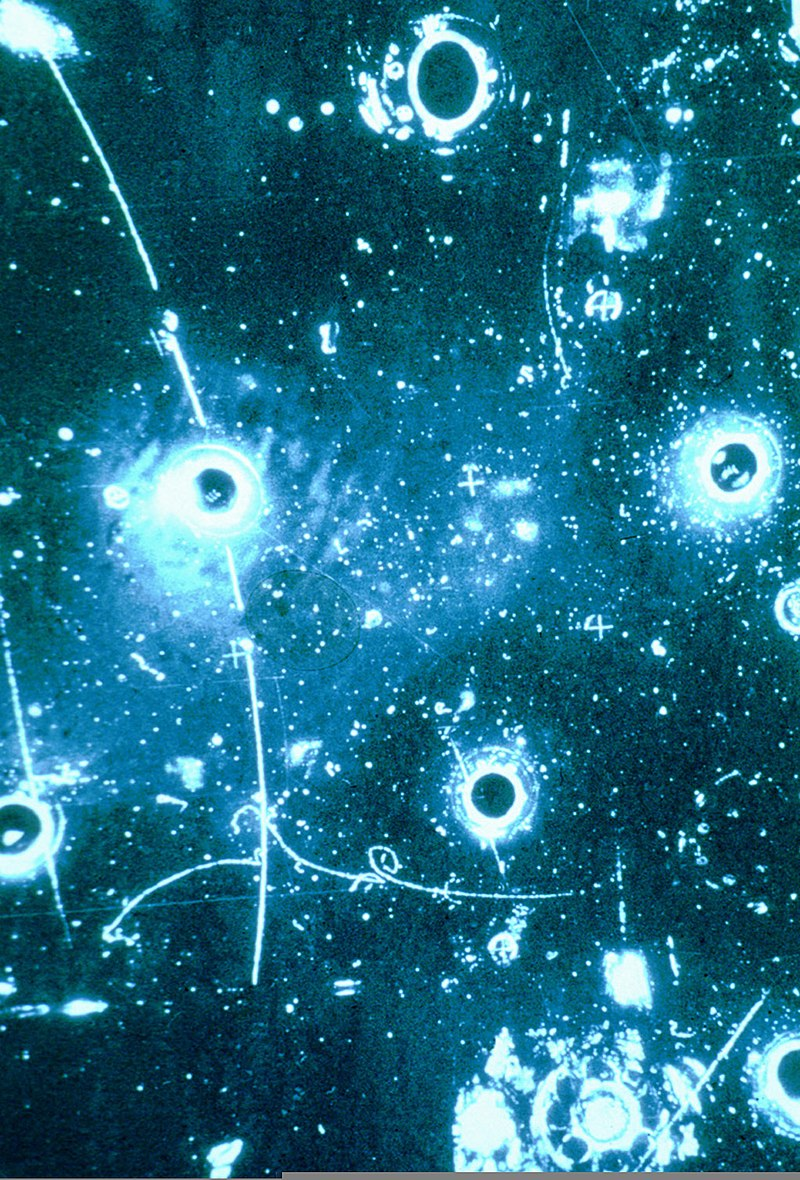
\includegraphics[width=4.5cm]{Leptonic_event_in_Gargamelle_bubble_chamber.jpg}}
\end{picture} \\ Doç. Dr. Mesut Karakoç}


\date{\today}

\begin{document}

%% Turkish babel problem
%% https://tex.stackexchange.com/questions/160385/newgeometry-doesnt-work-with-turkish-babel-package
%%\shorthandoff{=}% Make = not active any more

\maketitle

\newpage

% change name to "İçindekiler"
\renewcommand{\contentsname}{İçindekiler}
\tableofcontents{}

\listoffigures
 
\listoftables

\newpage

{
\hspace{.5\textwidth}
\begin{minipage}{.5\textwidth}
\raggedleft
If all this damned quantum jumps were really to stay, I should be
sorry I ever got involved with quantum theory.

—Erwin Schrödinger
\cite{book:Ficek}

%% Latince için
%% post iacturam quis non sapit!
%% Who is not wise after he has lost something?
%% https://quizlet.com/23756827/latin-proverbs-h-flash-cards/
\end{minipage}
}

\setcounter{section}{3} %% THIS WILL BE DELETED when all chapters merged!
\section{Bir Boyutlu Potansiyeller}

Üç boyutlu bir evrende yaşıyor olmamıza rağmen, bir çok fiziksel olayı (hareketi) bir boyutlu olarak tanımlamak mümkündür. Bu nedenle bu bölümde klasik fiziğin açıklayamadığı fakat kuantum fiziğiyle çalışabildiğimiz bazı bir boyutlu sistemleri inceleyeceğiz.


\subsection{Basamak Potansiyeli}
%%
\begin{figure}[hbtp]
	\centering
	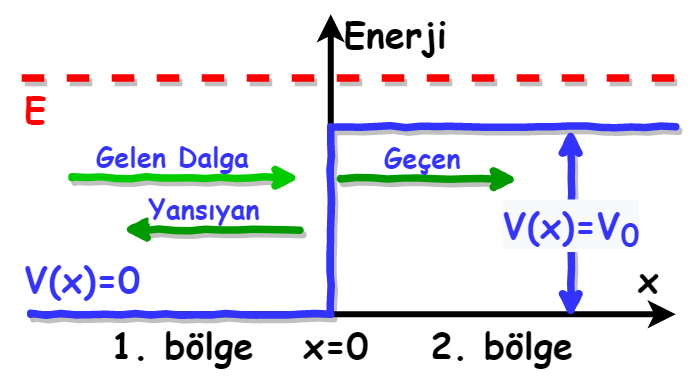
\includegraphics[width=0.7\linewidth]{figurler/Basamak_Potansiyeli}
	\caption{Basamak potansiyeli.}
	\label{fig:basamakpotansiyeli}
\end{figure}
%%
Basamak potansiyeli için bir örnek yukarıdaki şekildeki gibi olur. Şekilden anlaşılacağı üzere basamak potansiyeli; birbirinden farklı sabit potansiyellere sahip iki bölge içeren bir durumdur. Bir boyutlu hali için matematiksel ifadesi aşağıdaki gibidir.
%%
\begin{equation}
V ( x )  = \left\{ 
\begin{array} { l l } 
{ 0 } & {\Leftarrow x < 0 } \\ 
{ V _ { 0 } } & {\Leftarrow x \geq 0 } 
\end{array} \right. 
\end{equation}
%%

Bu potansiyeli zamandan bağımsız Schrödinger denklemi ile çalışabiliriz. Öncelikle Schrödinger denklemini yazılışı daha kolay olan,
%%
\begin{equation}
- \frac { \hbar ^ { 2 } } { 2 m } \frac { d ^ { 2 } u ( x ) } { d x ^ { 2 } } + V ( x ) u ( x ) = E u ( x )
\end{equation}
%%
formuna dönüştürebiliriz.

\begin{equation}
\frac { d ^ { 2 } u ( x ) } { d x ^ { 2 } } + \frac { 2 m } { \hbar ^ { 2 } } [ E - V ( x ) ] u ( x ) = 0
\end{equation}
%%
Basamak potansiyelinin değerinin sıfır olduğu bölge için,
%%
\begin{equation}
\frac { 2 m} { \hbar ^ { 2 } } E = k ^ { 2 }
\end{equation}
%%
tanımını ve sıfırdan farklı olduğu bölge için
%%
\begin{equation}
\frac { 2 m} { \hbar ^ { 2 } }  \left( E - V _ { 0 } \right) = q ^ { 2 }
\end{equation}
%%
tanımını yapabiliriz. $x<0$ ve $V(x)=0$ bölgesi için çözüm
%%
\begin{equation}
u_1 ( x ) \equiv u ( x ) = A e ^ { i k x } + B e ^ { - i k x }
\end{equation}
%%
olarak yazılabilir. Burada $A e ^ { i k x }$, $x=-\infty$'deki bir kaynaktan gelen serbest düzlem dalga olarak düşünülebilir, $B e ^ { -i k x }$ ise $x=0$ noktasında ortam değişikliğinden dolayı yansıyan dalga olarak düşünülebilir. Bu bölgedeki toplam olasılık akısı,
%%
\begin{equation}
\begin{array} { r l } 
{ j_1 } &\equiv  j  = \frac { \hbar } { 2 i m } \left( u ^ { * } \frac { d u } { d x } - \frac { d u ^ { * } } { d x } u \right) \\
& = \frac { \hbar } { 2 i m } \left[ \left(A^{*} e ^ { - i k x } + B ^ { * } e ^ { i k x } \right) \left(i k A e ^ { i k x } - i k B e ^ { - i k } \right) - \left( -i k A^{*} e ^ { -i k x } + i k B^* e ^ {  i k } \right) \left( A e ^ { i k x } + B  e ^ { -i k x } \right)  \right]  \\ 
{ } & { = \frac { \hbar k } { m } \left( | A | ^ { 2 }  - | B | ^ { 2 } \right) } \end{array}
\end{equation}
%%
olur. $x>0$ ve $V(x)=V_0$ için ise,
%%
\begin{equation}
u_2 ( x ) \equiv u ( x ) =  C e ^ { i q x }
\end{equation}
%%
çözümü elde edilir. Sadece $C e ^ { i q x }$ kısmı vardır, çünkü bu bölge $x=+\infty$'a kadar uzanmaktadır ve potansiyel sabittir bu yüzden, yansıyan dalga söz konusu değildir. Sadece $+x$ yönünde ilerleyen olasılık dalgası vardır. Bu olasılık dalgası için olasılık akısı,
%%
\begin{equation}
j_2 \equiv j = \frac { \hbar q } { m } | C | ^ { 2 }
\end{equation}
%%
bulunur. Her iki bölgedeki olasılık akıları ($j_1 = j_2$) birbirine eşit olmalıdır. Eğer,
%%
\begin{equation}
\frac { \partial } { \partial t } P ( x , t ) + \frac { \partial } { \partial x } j ( x , t ) = 0
\end{equation}
%%
olduğu hatırlanırsa ve kısmi değişkenlere ayrılabilir dalga fonksiyonu ile çalıştığımızdan $P(x, t) = \psi(x,t) \psi^*(x,t) = u(x) u^*(x)$ olacağına göre,
%%
\begin{equation}\label{key}
\frac { \partial } { \partial t } P ( x , t ) = \frac { \partial } { \partial t } |u ( x)|^2 = 0
\end{equation}
%%
elde edilir. Buradan,
%%
\begin{equation}
\frac { \partial } { \partial x } j ( x , t ) = 0
\end{equation}
%%
sonucuna ulaşırız. $x=0$ civarında $x=\pm\varepsilon \rightarrow 0$ aralığında yukarıdaki ifadenin integrali,
%%
\begin{equation}
\int^{\varepsilon}_{-\varepsilon} dx \frac { \partial } { \partial x } j ( x , t ) = j (\varepsilon  , t ) - j ( -\varepsilon , t ) = 0
\end{equation}
%%
sonucunu verir. Böylece $j_1 = j_2$ olması gerektiği ortaya çıkar. Her iki bölgedeki olasılık akıları da $x$'ten bağımsız olduklarından sınırda eşitlerse bütün tanımlı uzay boyunca birbirlerine eşit olmalıdırlar,
%%
\begin{equation}
\frac { \hbar k } { m } \left( 1 - | R | ^ { 2 } \right) = \frac { \hbar q } { m } | T | ^ { 2 }
\end{equation}
%%
yukarıdaki eşitlikle bu sonuç ifade edilmiş olur. Böylece bu tür sistemler için olasılık akısının bir 


\begin{equation}
1 + R = T
\end{equation}



\begin{equation}
\begin{array} { r l } { \left( \frac { d u } { d x } \right) _ { s } - \left( \frac { d u } { d x } \right) _ { - \varepsilon } } & { = \int _ { - \varepsilon } ^ { \varepsilon } d x \frac { d } { d x } \frac { d u } { d x } } \\ { } & { = \int _ { - s } ^ { s } d x \frac { 2 m } { \hbar ^ { 2 } } [ V ( x ) - E ] u ( x ) = 0 } \end{array}
\end{equation}




\begin{equation}
\begin{aligned} \left( \frac { d u } { d x } \right) _ { a + s } - \left( \frac { d u } { d x } \right) _ { a - s } & = \frac { 2 m } { \hbar ^ { 2 } } \int _ { a - s } ^ { a + s } d x \lambda \delta ( x - a ) u ( x ) \\ & = \frac { 2 m } { \hbar ^ { 2 } } \lambda u ( a ) \end{aligned}
\end{equation}


\begin{equation}
i k ( 1 - R ) = i q T
\end{equation}


\begin{equation}
\begin{array} { l } { R = \frac { k - q } { k + q } } \\ { T = \frac { 2 k } { k + q } } \end{array}
\end{equation}


\begin{equation}
\begin{array} { l } { \frac { \hbar k } { m } | R | ^ { 2 } = \frac { \hbar k } { m } \left( \frac { k - q } { k + q } \right) ^ { 2 } } \\ { \frac { \hbar q } { m } | T | ^ { 2 } = \frac { \hbar k } { m } \frac { 4 k q } { ( k + q ) ^ { 2 } } } \end{array}
\end{equation}


\begin{equation}
u ( x ) = T e ^ { - | q | x }
\end{equation}


\begin{equation}
| R | ^ { 2 } = \left( \frac { k - i | q | } { k + i | q | } \right) \left( \frac { k - i | q | } { k + i | q | } \right) ^ { * } = 1
\end{equation}


\begin{equation}
T = \frac { 2 k } { k + i | q | }
\end{equation}


\subsection{Sonlu Potansiyel Kuyusu}

\newpage
% In the preamble, add "\renewcommand\refname{New Title}" for article type documents 
% and "\renewcommand\bibname{New Title}" for book and report type documents.
\renewcommand\refname{Kaynaklar}
\bibliography{quantumBIB}{}
%% https://www.sharelatex.com/learn/latex/bibtex_bibliography_styles
 \bibliographystyle{plain}
%% \bibliographystyle{alpha}
%%\bibliographystyle{apalike}
\end{document}

